\documentclass{beamer}
\usepackage{bookmark}
\usepackage{pifont}
\usepackage{booktabs}
\usepackage{tikz}
\usepackage{adjustbox}
\usepackage{float}
\usepackage{longtable}
\usepackage{subcaption}
\usepackage{amsfonts}
\usepackage{ragged2e}
\usepackage{color, colortbl}
% Otros aportes y porcentaje en los objetivos 
\usepackage[spanish,mexico]{babel}
\usepackage[spanish]{algorithm2e}
\usepackage{media9}
\usepackage[duration=25,lastminutes=5]{pdfpcnotes}
\title{Examen de grado}
\subtitle{Despliegue en Hardware de un Sistema de Diagnóstico
Asistido por Computadora basado en Deep Learning para la
clasificación y detección de células de cáncer cervicouterino
en un examen de Papanicolau}
\author[Marco del Moral]{Marco Julio del Moral Argumedo \\ Alberto Aguilar Laserre \\ Rubén Posada Gómez}
\institute[ITO]{Tecnológico Nacional de México/Instituto Tecnológico de Orizaba}
\date{12/Diciembre/2019}

\definecolor{LightCyan}{rgb}{0.88,1,1}
\definecolor{titlepagecolor}{cmyk}{1,.60,0,.40}
\definecolor{namecolor}{cmyk}{1,.50,0,.10}
\definecolor{portadaa}{RGB}{73, 86, 120}
\definecolor{azul}{rgb}{0.768, 0.729, 0.949}
\definecolor{verde}{rgb}{0.847, 0.949, 0.729}
\definecolor{media}{rgb}{0.909, 0.670, 0.886} 
\newcommand\insertlogoii{}
\newcommand\logoii[1]{\renewcommand\insertlogoii{#1}}

\usetheme[]{Berkeley}    % JuanLesPins Berkeley PaloAlto Warsaw Goettingen Marburg
\usefonttheme{professionalfonts} % default professionalfonts serif structurebold structureitalicserif structuresmallcapsserif
\usecolortheme{whale} % albatross beaver beetle crane dolphin fly lily orchid rose seahorse seagull whale default
\useinnertheme{rectangles}
\setbeamerfont{section in sidebar}{size=\fontsize{5}{6}\selectfont}
\setbeamerfont{subsection in sidebar}{size=\fontsize{4}{5}\selectfont}
\setbeamerfont{subsubsection in sidebar}{size=\fontsize{3}{4}\selectfont}
\makeatletter

\setbeamertemplate{footline}
        {
      \leavevmode%
      \hbox{%
      \begin{beamercolorbox}[wd=.333333\paperwidth,ht=2.2ex,dp=1ex,center]{author in head/foot}%
        \usebeamerfont{author in head/foot}marcojulioarg@gmail.com
      \end{beamercolorbox}%
      \begin{beamercolorbox}[wd=.333333\paperwidth,ht=2.2ex,dp=1ex,center]{title in head/foot}%
        \usebeamerfont{title in head/foot}\insertshorttitle
      \end{beamercolorbox}%
      \begin{beamercolorbox}[wd=.333333\paperwidth,ht=2.2ex,dp=1ex,center]{date in head/foot}%
        \usebeamerfont{date in head/foot}\insertframenumber\,/\,\inserttotalframenumber%\hspace*{2em}

    %#turning the next line into a comment, erases the frame numbers
        %\insertframenumber{} / \inserttotalframenumber\hspace*{2ex} 

      \end{beamercolorbox}}%
      \vskip0pt%
    }

\setbeamertemplate{headline}
    {%
      \begin{beamercolorbox}[wd=\paperwidth]{frametitle}
        \ifx\beamer@sidebarside\beamer@lefttext%
        \else%
          \hfill%
        \fi%
        \ifdim\beamer@sidebarwidth>0pt%  
          \usebeamercolor[bg]{logo}%
          \vrule width\beamer@sidebarwidth height \beamer@headheight%
          \hskip-\beamer@sidebarwidth%
          \hbox to \beamer@sidebarwidth{\hss\vbox to
            \beamer@headheight{\vss\hbox{\color{fg}\insertlogo}\vss}\hss}%
          \hfill%
          \vrule width\beamer@sidebarwidth height \beamer@headheight%
          \hskip-\beamer@sidebarwidth%
          \hbox to \beamer@sidebarwidth{\hss\vbox to
            \beamer@headheight{\vss\hbox{\color{fg}\insertlogoii}\vss}\hss}%
        \else%
          \vrule width0pt height \beamer@headheight%  
        \fi%
      \end{beamercolorbox}
  }
  \makeatother
  \makeatletter
    \setbeamertemplate{sidebar \beamer@sidebarside}%{sidebar theme}
    {
      \beamer@tempdim=\beamer@sidebarwidth%
      \advance\beamer@tempdim by -6pt%
      \insertverticalnavigation{\beamer@sidebarwidth}%
      \vfill
      \ifx\beamer@sidebarside\beamer@lefttext%
      \else%
        \usebeamercolor{normal text}%
        \llap{\usebeamertemplate***{navigation symbols}\hskip0.1cm}%
        \vskip2pt%
      \fi%
  }%
  \makeatother

\graphicspath{ {imagenes/} }

\logo{\includegraphics[height=1cm]{logo_transparente}}
\logoii{\includegraphics[height=1cm]{CONACYT1-2}}


\begin{document}

    \begin{frame}
        \titlepage{}
        \note{Ser muy breve.}
        \note{Presentaré los avances de la tesis titulada.}
    \end{frame}

    \section{Introducción}

    % \begin{frame}{El flagelo de la humanidad}{¿Qué es el cáncer?}
    %     \begin{figure}[]
    %         \centering
    %         \includegraphics[width=1\textwidth]{celu.png}
    %         % \caption{Desarrollo del cáncer}\label{fig:desarrollo}
    %     \end{figure}
    %     \pnote{Crecimiento anormal de células.}
    %     \pnote{Dañó genético por múltiples causas.}
    %     \pnote{Una enfermedad difícil de vivir y de tratar.}

    % \end{frame}

    \begin{frame}{El Cáncer Cérvicouterino}{Factores y síntomas}
        \begin{figure}[]
            \centering
            \includegraphics[height=0.95\textheight]{secretaria}
            % \caption{Desarrollo del cáncer}\label{fig:desarrollo}
        \end{figure}
        \pnote{Manuscritos en Egipto de hace 4000 años, no había tratamiento.}
        \pnote{Es del sexo femenino.}
        \pnote{Se localiza en el cuello del cérvix.}
        \pnote{Sus síntomas son.}
        \pnote{Factores de riesgo: VPH.}
        \pnote{Como podemos ver, hay esfuerzos gubernamentales.}
    \end{frame}

    \begin{frame}{El Cáncer Cérvicouterino}{Datos y estadísticas}
        \begin{block}{Estadísticas}{
            \begin{itemize}
                \item La séptima neoplasia más frecuente a nivel mundial y la cuarta entre mujeres.
                \item 85\% de los casos son en países en vías de desarrollo.
                \item La tendencia de mortalidad es descendente.
                \item Es un indicador de la desigualdad.
                \item Primera causa de muerte por tumor en países en vías de desarrollo.
                % \item El 75\% de las defunciones en LA ocurren en seis países, incluido México.
                \item Segunda muerte por cáncer en la mujer mexicana.
                \item 14000 nuevos casos al año en México.
                \item 10 muertes por día, 4700 al año.
                % \item Se hacen en México 5 millones de pruebas citológicas.
            \end{itemize}
        }
        \end{block}
        \pnote{Como pueden ver, es un problema grande para nuestro pais.}
    \end{frame}

    \section{Planteamiento}
    \begin{frame}{El problema}{Proceso patológico}

        \begin{block}{Factores de prognosis}
            {
                \begin{itemize}
                    \item El cáncer es progresivo.
                    \item Es etapas avanzadas, es incurable.
                    \item Detección temprana es la primera defensa.
                \end{itemize}
            }
        \end{block}

        \begin{exampleblock}{Factores de diagnóstico}
            {
                \begin{itemize}
                    \item Se toma una muestra del paciente
                    \item Se usa microscopio para el diagnóstico.
                    \item Se realiza un análisis morfológico.
                \end{itemize}
            }
        \end{exampleblock}
        \pnote{Prognosis se refiere a las probabilidades de sobrevivir.}
        \pnote{Grandes razgos del proceso de diagnóstico}
    \end{frame}

    \begin{frame}{El problema}{Condiciones del diagnóstico}
        
        \begin{alertblock}{Incidencias negativas en la eficacia}{
            \begin{itemize}
                \item Se generan cinco millones de muestras al año.
                \item Poco personal para el diagnóstico.
                \item Error humano en la toma de muestras.
                \item Error humano por fatiga y sobretrabajo.
                \item Deterioro en la visión.
                \item Subjetividad e incertidumbre inherentes al proceso humano.
            \end{itemize}
        }
        \end{alertblock}
        \pnote{Variabilidad entre la tinción}
        \pnote{Dos personas para toda la región veracruz sur, cientos de muestras tomadas al día}
        \pnote{Se quedan ciegos}
        \pnote{Se levantó de malas, le duele la panza}
    \end{frame}

    \section{Propuesta}
    \begin{frame}{Propuesta}{Sistema de Diagnóstico Asistido por Computadora}
        \begin{figure}[]
            \centering
            \includegraphics[height=0.95\textheight]{diagrama_sistema}
        \end{figure}
        \pnote{SDAC implementado en un SE usando ML}
        \pnote{Uso dentro del laboratorio}
        \pnote{Asistir al experto}
    \end{frame}

    % \begin{frame}{Machine Learning}{Un nuevo paradigma}
    %     \tikzset{every picture/.style={line width=0.75pt}} %set default line width to 0.75pt        
    %     \begin{figure}[H]
    %         \centering  
        
    %         \begin{tikzpicture}[x=0.75pt,y=0.75pt,yscale=-1,xscale=1]
    %         %uncomment if require: \path (0,300); %set diagram left start at 0, and has height of 300
            
    %         %Shape: Rectangle [id:dp5656002629863663] 
    %         \draw   (331.05,93.82) -- (419.15,93.82) -- (419.15,149.34) -- (331.05,149.34) -- cycle ;
    %         %Shape: Rectangle [id:dp08469876048021208] 
    %         \draw   (331.05,10.55) -- (419.15,10.55) -- (419.15,66.06) -- (331.05,66.06) -- cycle ;
    %         %Right Arrow [id:dp5526832475614203] 
    %         \draw   (431.74,33.07) -- (448.91,33.07) -- (448.91,27.62) -- (460.35,38.51) -- (448.91,49.41) -- (448.91,43.96) -- (431.74,43.96) -- cycle ;
    %         %Right Arrow [id:dp11323285532946126] 
    %         \draw   (430.48,114.95) -- (447.65,114.95) -- (447.65,109.5) -- (459.09,120.4) -- (447.65,131.29) -- (447.65,125.85) -- (430.48,125.85) -- cycle ;
    %         %Striped Right Arrow [id:dp37446377869018366] 
    %         \draw   (298.39,11.9) -- (311.21,11.9) -- (311.21,6.8) -- (323.16,17) -- (311.21,27.2) -- (311.21,22.1) -- (298.39,22.1) -- cycle ;\draw   (293.29,11.9) -- (294.31,11.9) -- (294.31,22.1) -- (293.29,22.1) -- cycle ;\draw   (295.33,11.9) -- (297.37,11.9) -- (297.37,22.1) -- (295.33,22.1) -- cycle ;
    %         %Striped Right Arrow [id:dp511490599188687] 
    %         \draw   (298.39,53.54) -- (311.21,53.54) -- (311.21,48.44) -- (323.16,58.64) -- (311.21,68.84) -- (311.21,63.74) -- (298.39,63.74) -- cycle ;\draw   (293.29,53.54) -- (294.31,53.54) -- (294.31,63.74) -- (293.29,63.74) -- cycle ;\draw   (295.33,53.54) -- (297.37,53.54) -- (297.37,63.74) -- (295.33,63.74) -- cycle ;
    %         %Striped Right Arrow [id:dp24056201288099344] 
    %         \draw   (297.13,96.56) -- (309.95,96.56) -- (309.95,91.46) -- (321.9,101.66) -- (309.95,111.86) -- (309.95,106.76) -- (297.13,106.76) -- cycle ;\draw   (292.03,96.56) -- (293.05,96.56) -- (293.05,106.76) -- (292.03,106.76) -- cycle ;\draw   (294.07,96.56) -- (296.11,96.56) -- (296.11,106.76) -- (294.07,106.76) -- cycle ;
    %         %Striped Right Arrow [id:dp09567701368722925] 
    %         \draw   (297.13,138.2) -- (309.95,138.2) -- (309.95,133.1) -- (321.9,143.3) -- (309.95,153.5) -- (309.95,148.4) -- (297.13,148.4) -- cycle ;\draw   (292.03,138.2) -- (293.05,138.2) -- (293.05,148.4) -- (292.03,148.4) -- cycle ;\draw   (294.07,138.2) -- (296.11,138.2) -- (296.11,148.4) -- (294.07,148.4) -- cycle ;
            
            
    %         % Text Node
    %         \draw (375.1,38.31) node [scale=0.8] [align=left] {Programación\\Clásica};
    %         % Text Node
    %         \draw (375.1,121.58) node [scale=0.8] [align=left] {Machine\\Learning};
    %         % Text Node
    %         \draw (271.89,16.1) node [scale=0.8] [align=left] {Reglas};
    %         % Text Node
    %         \draw (483.34,118.8) node [scale=0.8] [align=left] {Reglas};
    %         % Text Node
    %         \draw (273.78,100.76) node [scale=0.8] [align=left] {Datos};
    %         % Text Node
    %         \draw (273.78,59.12) node [scale=0.8] [align=left] {Datos};
    %         % Text Node
    %         \draw (261.19,143.78) node [scale=0.8] [align=left] {Respuestas};
    %         % Text Node
    %         \draw (494.04,36.92) node [scale=0.8] [align=left] {Respuestas};
            
    %         \end{tikzpicture}
    %     \end{figure}
    %     \pnote{Programación clásica = lógica difusa}
    % \end{frame}

    \begin{frame}{Deep Learning}{Aprendizaje jerárquico}
        \begin{figure}[]
            \centering
            \includegraphics[width=\textwidth]{comparacion}
        \end{figure}
        \pnote{Ahora no se requiere una fase costosa de extracción de características}
        \pnote{Se refiere a algoritmos especiales para extraer información de una imagen}
    \end{frame}

    \begin{frame}{Deep Learning}{El poder de las Redes Neuronales Convolucionadas}
        \begin{figure}[]
            \centering
            \includegraphics[width=\textwidth]{arch}
        \end{figure}
        \pnote{Es una red que puede recibir datos volumétricos, como una imagen RGB}
        \pnote{En cada paso va concentrado la información, por lo que se requieren menos parámetros}
    \end{frame}

    \begin{frame}{ConvNets}{Aplicaciones y alcance}
        \begin{figure}[]
            \centering
            \includegraphics[width=\textwidth]{oristarry}
        \end{figure}
        \pnote{Ejemplos: Carros autónomos, etiquetado de fotos en FB, filtros}
        \pnote{Reconocimiento de voz, procesamiento de lenguaje natural}
        \pnote{Inclusive arte, como en la música o Neural Style Transfer}
    \end{frame}

    % \begin{frame}{ConvNets}{Obras de arte}
    %     \begin{figure}[]
    %         \centering
    %         \includegraphics[width=\textwidth]{marcostarry}
    %     \end{figure}
    % \end{frame}

    \section{Desarrollo}
    \begin{frame}{Metodología}{Un enfoque secuencial de transformación}
        \begin{figure}[]
            \centering
            \includegraphics[width=1\textwidth]{metodologia_basica_final}
        \end{figure}
        \pnote{Son 7 pasos generales para proyectos de ML}
        \pnote{Se transforma una problemática en un sistema}
    \end{frame}

    \subsection{Análisis general}
    % \subsubsection{Definir el problema}
    \begin{frame}{Definir el problema}{Detectar y clasificar células cervicales}
        \begin{figure}[]
            \centering
            \includegraphics[width=1\textwidth]{papsmear.jpg}
            % \caption{Prueba de Papanicolau}\label{fig:papsmear}
        \end{figure}
        \pnote{Se toma una muestra del examen Pap}
        \pnote{Se analiza la laminilla en el microscopio}
    \end{frame}

    \begin{frame}{Definir el problema}{Relación entre el daño celular y el cáncer}
        \begin{figure}[]
            \centering
            \includegraphics[height=1\textheight]{ciclo.jpg}
        \end{figure}
        \pnote{La morfología celular da el tipo de lesión}
    \end{frame}

    % \subsubsection{Búsqueda de soluciones previas}
    % \begin{frame}{Búsqueda de soluciones previas}{AutoCyte}
    %     \begin{figure}[]
    %         \centering
    %         \includegraphics[width=1\textwidth]{autocyte}
    %         % \caption{Prueba de Papanicolau}\label{fig:papsmear}
    %     \end{figure}
    %     \note{30 veces más caro que las pruebas normales}
    % \end{frame}
    % \subsubsection{Determinar tipo de problema}
    \begin{frame}{Determinar tipo de problema}{ConvNets aplicadas a visión por computadora}
        \begin{figure}[]
            \centering
            \includegraphics[width=\textwidth]{tipos}
          \end{figure}
          \pnote{Pixeles, mono objeto y multiobjeto}
    \end{frame}
    % \subsubsection{Generación de supuestos}
    \begin{frame}{Generación de supuestos}{El sustento de toda investigación}
        \begin{block}{Supuestos metodológicos}{
            \begin{itemize}
                \item El núcleo celular contiene suficiente información para
                diferenciar entre los tipos de célula citológica cervical.
                \item Las técnicas de aumento de datos no inciden en la decisión
                del algoritmo.
                % \item La red neuronal es capaz de diferenciar correctamente en
                % un espacio multidimensional entre los tipos de célula.
            \end{itemize}
        }
        \end{block}
        \pnote{Permiten sustentar la investigación delimitando el espacio de soluciones}
    \end{frame}

    \subsection{Obtención de datos}
    \begin{frame}{DTU/Herlev dataset}{Hospital Universitario de Herlev | Universidad del Mar Egeo}

        \begin{columns}
            \column{.5\textwidth}
            \includegraphics[width=\columnwidth,height=\columnwidth]{herlev}
    
            \column{.5\textwidth}
            \begin{block}{Compiladores}{
                \begin{itemize}
                    \item Jan Jantzen.
                    \item G. Dounnias.
                \end{itemize}
            }   
            \end{block}
            \begin{exampleblock}{Características}{
                \begin{itemize}
                    \item Imágenes clasificadas y validadas.
                    \item Análisis realizado por un conjunto de expertos.
                    \item Tesis y artículos que usan la base de datos.
                \end{itemize}
            }
            \end{exampleblock}
        \end{columns}
        \pnote{Fueron muy amables}
        \pnote{Estuvieron pendientes para cualquier duda}
        \pnote{Validación: conjunto de expertos, si uno discrepaba se elimina la imagen}
    \end{frame}

    \subsection{Exploración}
    \begin{frame}{Análisis de atributos}{Conteo de clases y categorías}
        \begin{table}
            \centering
            \resizebox{\textwidth}{!}{%
            \begin{tabular}{@{}lllll@{}}
            \toprule
            Clase & Categoría & Clase & Cantidad & Subtotales \\ \midrule
            0 & Normal & Superficial squamous epithelial & 74 &  \\
            1 & Normal & Intermediate squamous epithelial & 70 &  \\
            2 & Normal & Columnar epithelial & 98 & 242 normales \\ \midrule
            3 & Anormal & Mild squamous non-keratinizing dysplasia & 182 &  \\
            4 & Anormal & Moderate squamous non-keratinizing dysplasia & 146 &  \\
            5 & Anormal & Severe squamous non-keratinizing dysplasia & 197 &  \\
            6 & Anormal & Squamous cell carcinoma in situ intermediate & 150 & 675 anormales \\ \bottomrule
              &         &                                              &     & 917 totales
            \end{tabular}%
            }
            \end{table}
            \pnote{7 clases, 2 categorías}
            \pnote{Basado en sistema bethesda}
            \pnote{Células epiteliales y escamosas}
    \end{frame}
    % \subsubsection{Análisis de atributos}
    \begin{frame}{Visualización}{Muestras de células}
        \begin{figure}[]
            \centering
            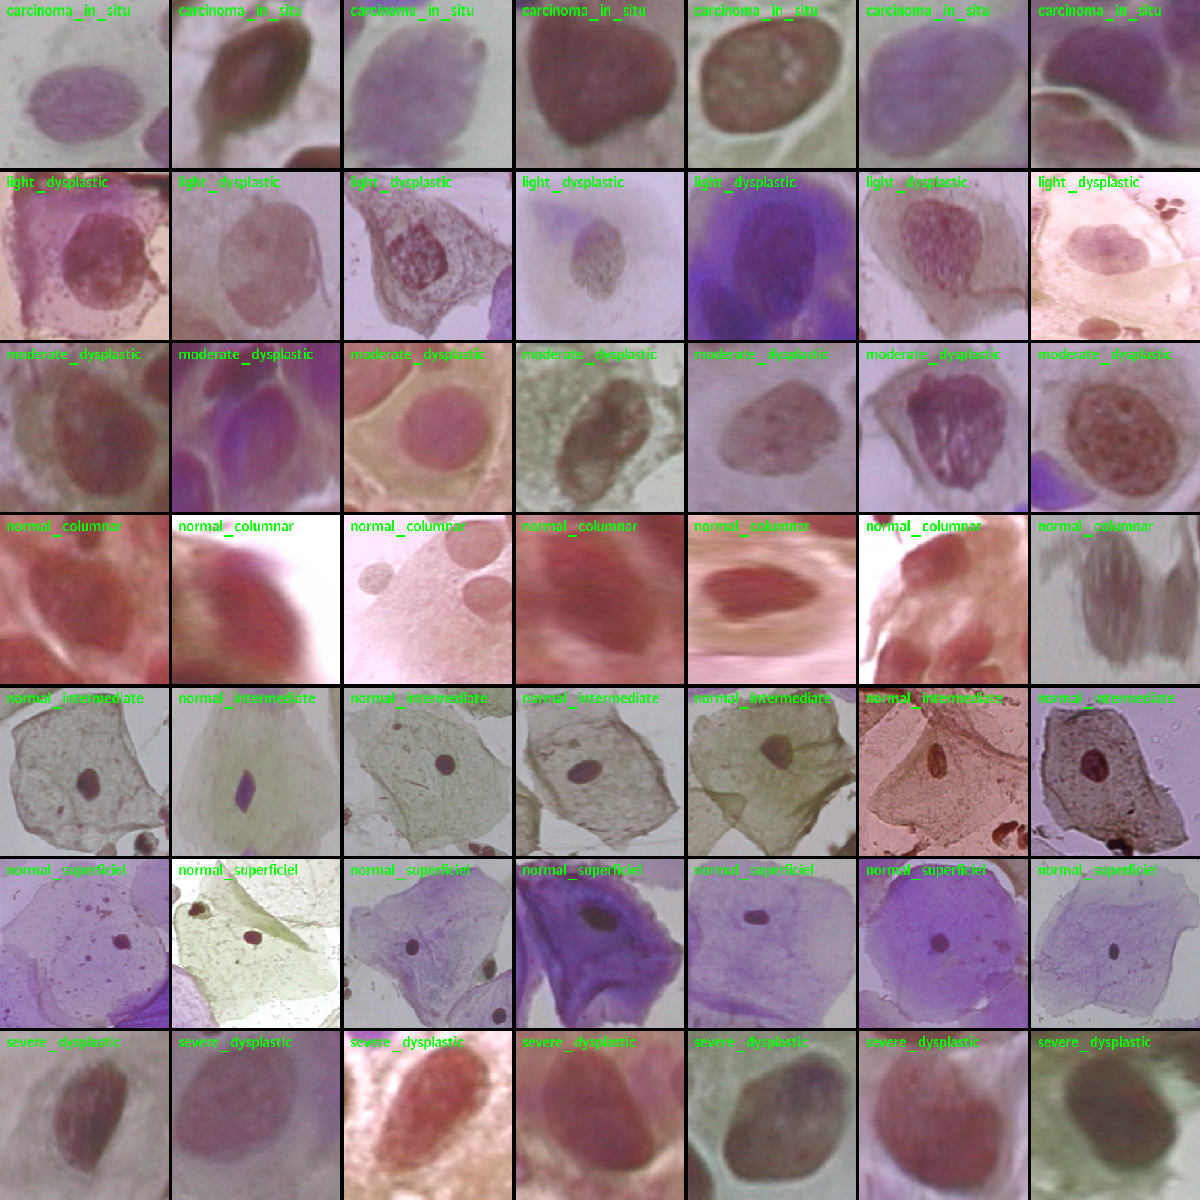
\includegraphics[height=0.9\textheight]{muestras_celulas}
        \end{figure}
        

    \end{frame}
    % \subsubsection{Aplicar estadística}
    \begin{frame}{Visualización}{Muestras de máscaras}
        \begin{figure}[]
            \centering
            \includegraphics[height=0.9\textheight]{muestras_mascaras}
        \end{figure}
    \end{frame}

    % \begin{frame}{Transformaciones aplicables}{Simetrías}
    %     \begin{figure}[]
    %         \centering
    %         \includegraphics[width=1\textwidth]{simetrias}
    %     \end{figure}
    % \end{frame}

    \subsection{Preprocesamiento}
    \begin{frame}{Aumentación de datos}{Proceso de aumentación}
        \begin{figure}[]
            \centering
            \includegraphics[width=1\textwidth]{augment}
        \end{figure}
    \end{frame}

    \begin{frame}{Aumentación de datos}{Resultados}
        \begin{figure}[]
            \centering
            \includegraphics[height=0.9\textheight]{muestras_augment}
        \end{figure}
        \pnote{Hay que ver si la aumentación afecta}
    \end{frame}

    \subsection{Elección algorítmica}
    \begin{frame}{\emph{Transfer Learning}}{Máquinas que aprenden del pasado}
        \begin{figure}[]
            \centering
            \includegraphics[width=1\textwidth]{transfer}
        \end{figure}
        \pnote{Redes preentrenadas en millones de imágenes}
        \pnote{Se transfieren los pesos de las capas iniciales y se añade un clasificador nuevo}
    \end{frame}

    % \begin{frame}{\emph{Transfer Learning}}{Pérdida en entrenamiento}
    %     \begin{figure}[]
    %         \centering
    %         \includegraphics[width=1\textwidth]{perdida_entrenamiento}
    %     \end{figure}
    %     \pnote{Se probaron muchas arquitecturas}
    %     \pnote{Al parecer todas se comportan bien}
    % \end{frame}

    \begin{frame}{\emph{Transfer Learning}}{Pérdida en validación}
        \begin{figure}[]
            \centering
            \includegraphics[width=1\textwidth]{perdida_validacion}
        \end{figure}
        \pnote{En validación vemos que solo dos tienen buen rendimiento.}
    \end{frame}

    \subsection{Ajuste de modelo}
    \begin{frame}{Ajuste del modelo}{Dos tipos de experimentos posibles dada la base de datos}
        \begin{exampleblock}{Tipos de experimento}{
            \begin{enumerate}
                % \item{\textbf{Clasificación binaria:}} Clasificar las imágenes citológicas
                % en normales y anormales.
                \item{\textbf{Clasificación multi-clase:}} Clasificar las
                imágenes en las siete clases de la base de datos. Esta será el
                modelo que llegará a la solución final y por ello es el que
                lleva mayor cantidad de análisis.
                \item{\textbf{Segmentación semántica:}} Segmentar cada pixel de la imagen
                citológica en dos clases: núcleo o el resto (citoplasma o fondo).
            \end{enumerate}
        }
        \end{exampleblock}
    \end{frame}

    \begin{frame}{Validación cruzada}{Reducir la incertidumbre en la estimación del rendimiento}
        \begin{figure}[H]
            \centering
            \includegraphics[width=1\textwidth]{cross.pdf}
        \end{figure}
        \pnote{Permite evaluar correctamente el rendimiento}
        \pnote{Los pesos se inicializan de manera aleatoria, esto nos ayuda a reducir esa incertidumbre}
    \end{frame}

%     \begin{frame}{Clasificación binaria}{Tabla de resultados}
%         \begin{table}[H]
%             \centering
%             \resizebox{0.5\textwidth}{!}{%
%             \begin{tabular}{@{}lll@{}}
%             \toprule
%              & Exactitud & Pérdida \\ \midrule
%             Número & 10 & 10 \\
%             \rowcolor{azul}
%             Media & 99.86288667 & 0.003868326 \\
%             Desviación & 0.041250406 & 0.001303197 \\
%             Mínimo & 99.77319837 & 0.002261744 \\
%             25\% & 99.84793812 & 0.003078721 \\
%             50\% & 99.87113476 & 0.003741355 \\
%             75\% & 99.8865962 & 0.004018324 \\
%             Máximo & 99.91752505 & 0.006879645 \\ \bottomrule
%             \end{tabular}%
%             }
%             \end{table}
%     \end{frame}

%     \begin{frame}{Clasificación binaria}{Gráfica de pérdida}
%         \begin{figure}[]
%             \centering
%             \includegraphics[height=0.95\textheight]{reporte_2_class/loss.pdf}
%         \end{figure}
%     \end{frame}

%     \begin{frame}{Clasificación binaria}{Gráfica de exactitud}
% \begin{figure}[H]
%     \centering
%     \includegraphics[height=0.95\textheight]{reporte_2_class/acc.pdf}
% \end{figure}
%     \end{frame}

    \begin{frame}{Clasificación multi-clase}{Tabla de resultados}
        \begin{table}[H]
            \centering
            \resizebox{0.9\textwidth}{!}{%
            \begin{tabular}{@{}lll@{}}
            \toprule
             & Exactitud & Pérdida \\ \midrule
            Número & 10 & 10 \\
            \rowcolor{azul}
            Media & 99.58866 & 0.013302901 \\
            Desviación & 0.084239213 & 0.002258767 \\
            Mínimo & 99.46391582 & 0.009913217 \\
            25\% & 99.51546341 & 0.012080938 \\
            50\% & 99.60309267 & 0.013360192 \\
            75\% & 99.62371141 & 0.01459487 \\
            Máximo & 99.72165227 & 0.016523478 \\ \bottomrule
            \end{tabular}%
            }
            \end{table}
        \pnote{Se hace una validación de 10 veces}
    \end{frame}

    % \begin{frame}{Clasificación multi-clase}{Gráfica de pérdida}
    %     \begin{figure}[]
    %         \centering
    %         \includegraphics[height=0.95\textheight]{reporte_7_class/loss.pdf}
    %     \end{figure}
    % \end{frame}

    % \begin{frame}{Clasificación multi-clase}{Gráfica de exactitud}
    %     \begin{figure}[]
    %         \centering
    %         \includegraphics[height=0.95\textheight]{reporte_7_class/acc.pdf}
    %     \end{figure}
        
    % \end{frame}

    % \begin{frame}{Clasificación multi-clase}{Matriz de confusión normalizada}
    %     \begin{figure}[]
    %         \centering
    %         \includegraphics[height=0.95\textheight]{reporte_7_class/matriz_norm.pdf}
    %     \end{figure}
    % \end{frame}

    \begin{frame}{Clasificación multi-clase}{Matriz de confusión}
        \begin{figure}[]
            \centering
            \includegraphics[height=0.95\textheight]{reporte_7_class/matriz.pdf}
        \end{figure}
    \end{frame}

    % \begin{frame}{Clasificación multi-clase}{Curva ROC}
    %     \begin{figure}[H]
    %         \centering
    %         \includegraphics[height=0.95\textheight]{reporte_7_class/roc_multiclase.pdf}
    %     \end{figure} 
    % \end{frame}

    \begin{frame}{Clasificación multi-clase}{Reporte de clasificación tendencia 0}
        \begin{figure}[]
            \centering
            \includegraphics[height=0.95\textheight]{reporte_7_class/reporte_cero.pdf}
            
        \end{figure}
        \pnote{CEN = Entropía de confusión}
    \end{frame}

    \begin{frame}{Clasificación multi-clase}{Reporte de clasificación tendencia 1}
        \begin{figure}[]
            \centering
            \includegraphics[height=0.95\textheight]{reporte_7_class/reporte_uno.pdf}
        \end{figure}
        \pnote{BM = probabilidad de hacer una predicción correcta y no adivinar}
        \pnote{F1 = media armónica de la exactitud}
    \end{frame}

    % \begin{frame}{Clasificación multi-clase}{Muestreo de errores}
    %     \begin{figure}[]
    %         \centering
    %         \includegraphics[width=\textwidth]{reporte_7_class/muestras_erroneas.pdf}
    %     \end{figure}
    % \end{frame}

    \begin{frame}{Segmentación semántica}{Tabla de resultados}
        \begin{table}[H]
            \centering
            \resizebox{\textwidth}{!}{%
            \begin{tabular}{@{}llll@{}}
            \toprule
            & Exactitud & Pérdida & IoU \\ \midrule
            Número & 5 & 5 & 5 \\
            \rowcolor{azul}
            Media & 90.20958571 & -0.907671014 & 0.881990721 \\
            Desviación & 0.502696262 & 0.008608186 & 0.008644234 \\
            Mínimo & 89.79965767 & -0.s917515639 & 0.866708054 \\
            25\% & 89.86388168 & -0.911953644 & 0.884503568 \\
            50\% & 89.99839323 & -0.911352285 & 0.885264954 \\
            75\% & 90.36797129 & -0.900890709 & 0.885471006 \\
            Máximo & 91.0180247 & -0.896642793 & 0.888006022 \\ \bottomrule
            \end{tabular}%
            } 
            \end{table}
            \pnote{IOU = intersección sobre unión y se refiere a los pixeles}
    \end{frame}

    % \begin{frame}{Segmentación semántica}{Gráfica de pérdida}
    %     \begin{figure}[]
    %         \centering
    %         \includegraphics[height=0.95\textheight]{reporte_7_class/loss.pdf}
    %     \end{figure}
    % \end{frame}

    % \begin{frame}{Segmentación semántica}{Gráfica de IoU}
    %     \begin{figure}[]
    %         \centering
    %         \includegraphics[height=0.95\textheight, width=\textwidth]{exactitud_2}
    %     \end{figure}
        
    % \end{frame}

    \begin{frame}{Segmentación semántica}{Muestreo de validación}
        \begin{figure}[]
            \centering
            \includegraphics[height=0.95\textheight]{muestreo_mascaras_segmentacion}
        \end{figure}
        \pnote{Imagen, máscara, predicción, TP, FP, FN}
    \end{frame}

    % \begin{frame}{Segmentación semántica}{Muestreo de validación multi-objeto}
    %     \begin{figure}[]
    %         \centering
    %         \includegraphics[height=0.95\textheight]{test_segmentacion}
    %     \end{figure}
    % \end{frame}

    % \begin{frame}{Comprobación de supuestos}{Análisis de la primera capa}
    %     \begin{figure}[]
    %         \centering
    %         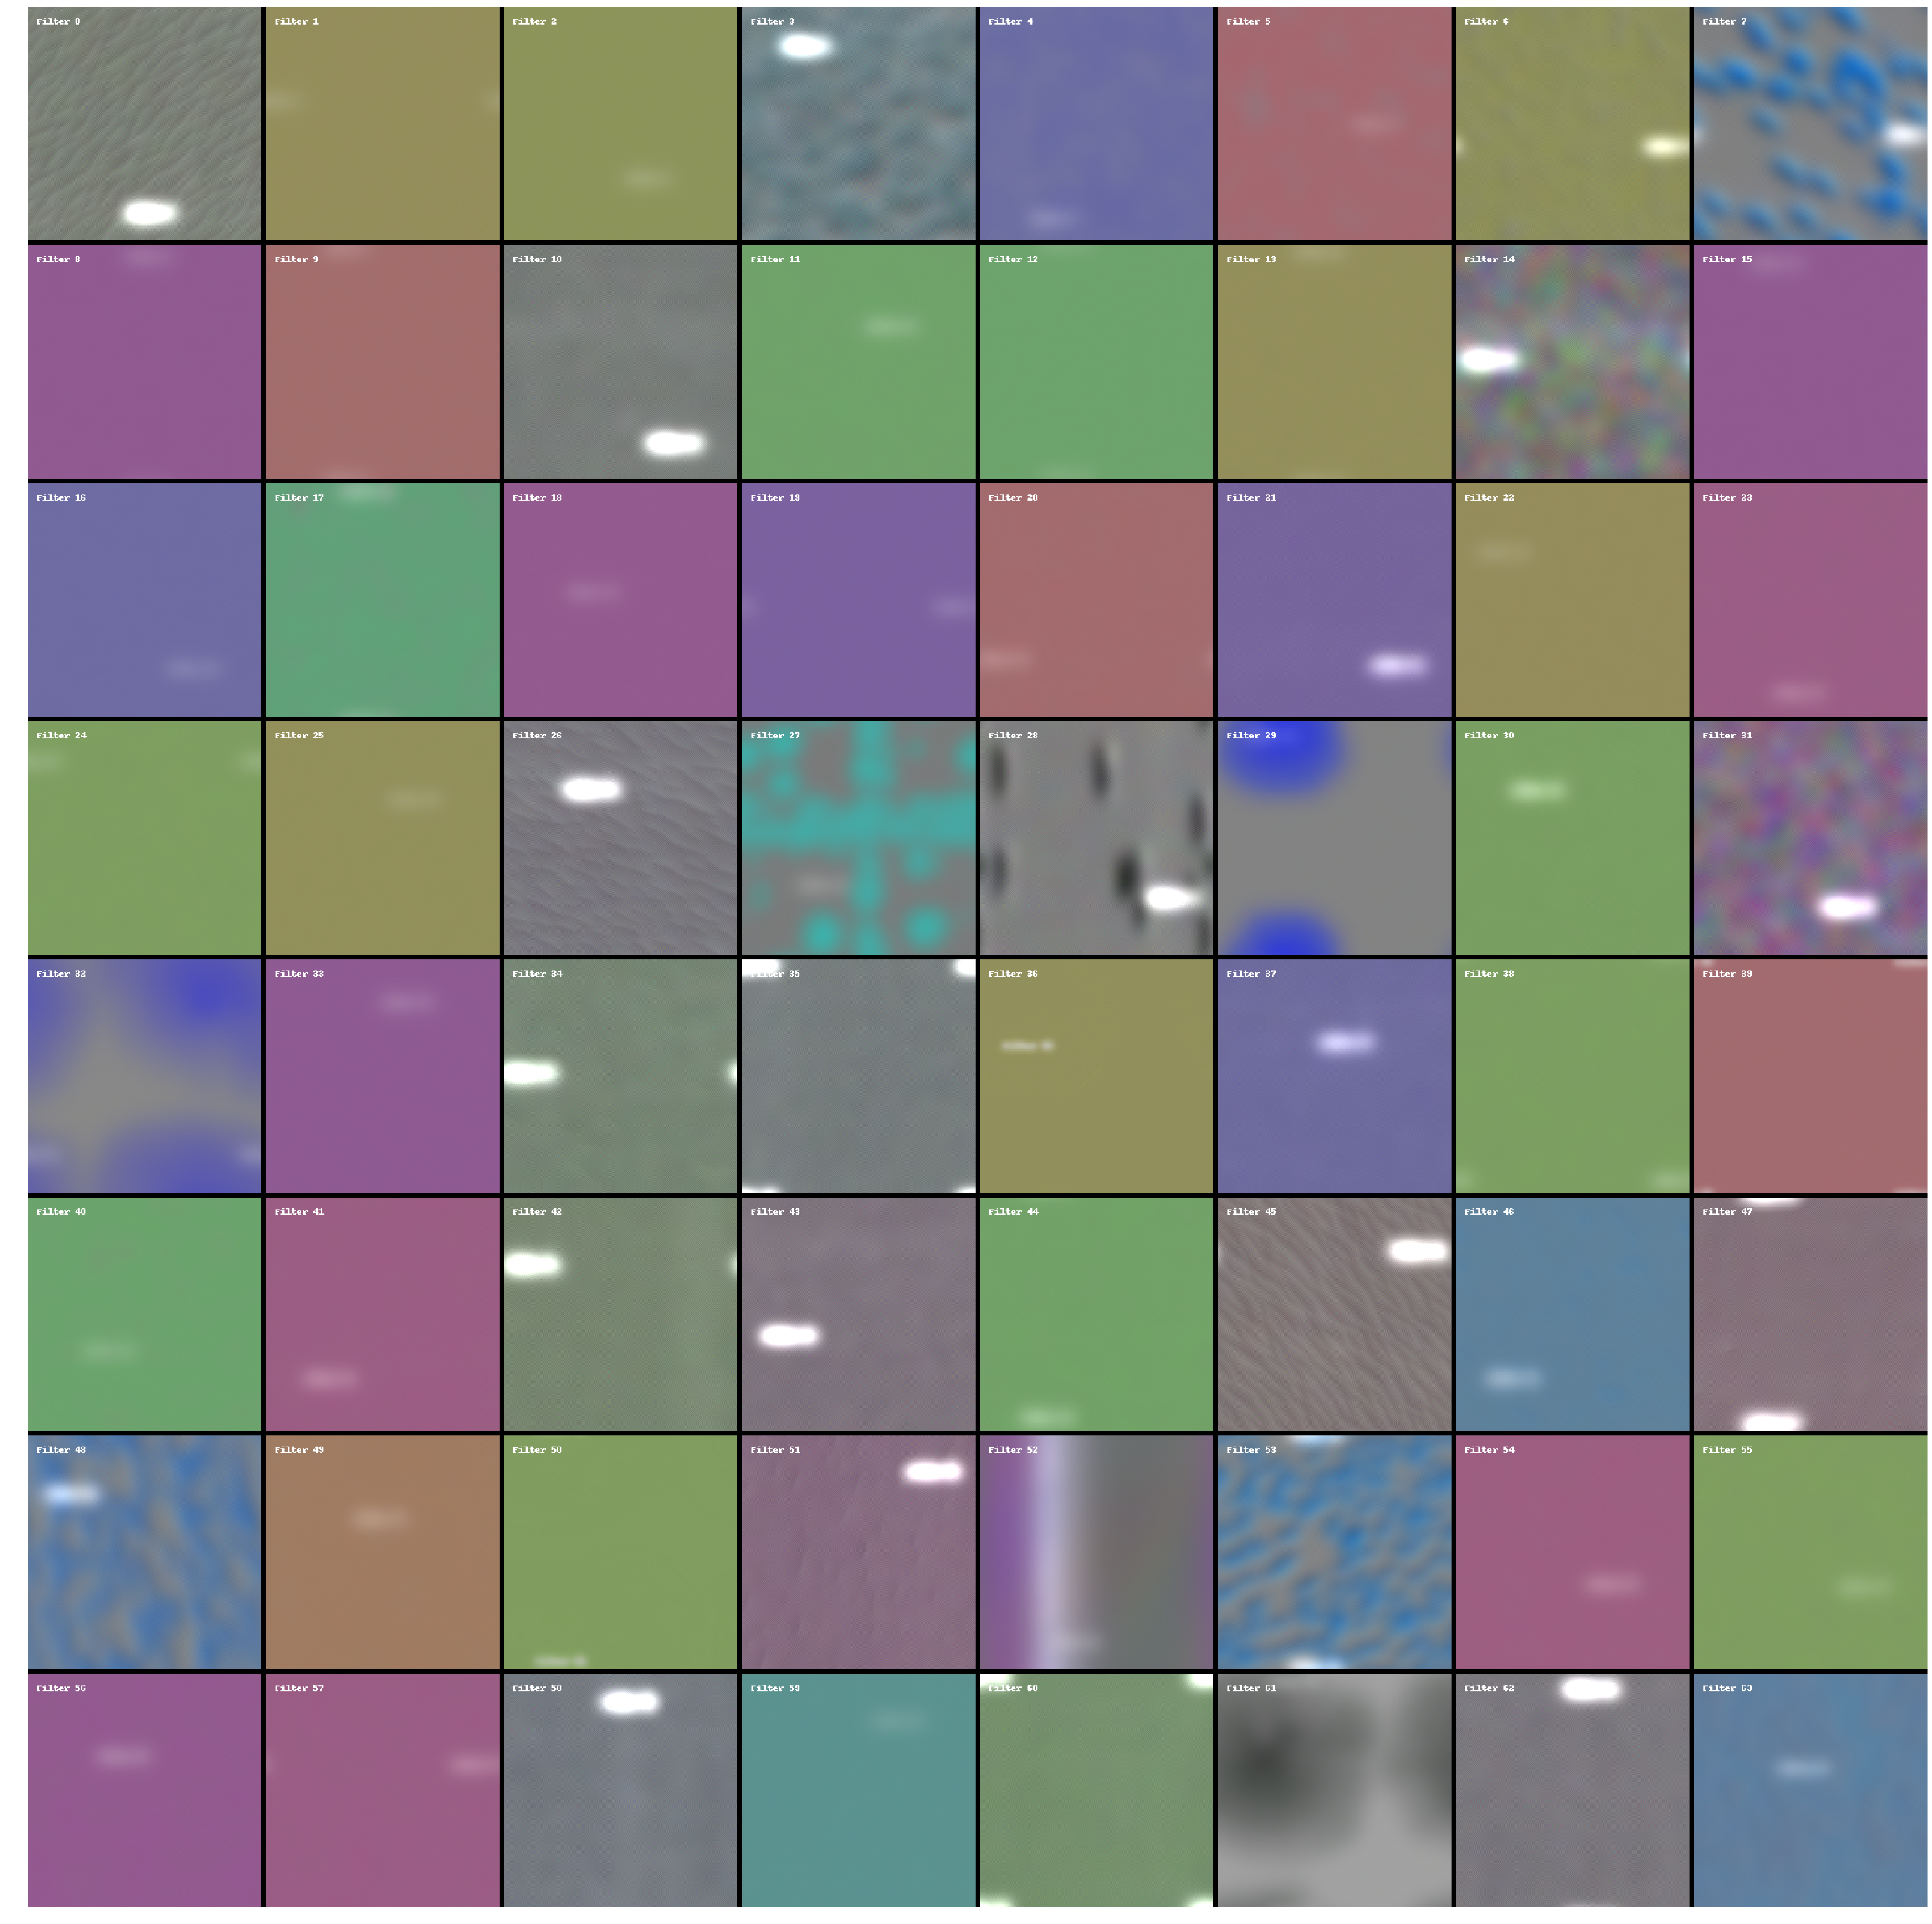
\includegraphics[height=0.95\textheight]{filtros-block1_conv1}
    %     \end{figure}
    %     \pnote{Identifica patrones sencillos como colores o bordes}
    % \end{frame}

    % \begin{frame}{Comprobación de supuestos}{Análisis de la última capa}
    %     \begin{figure}[]
    %         \centering
    %         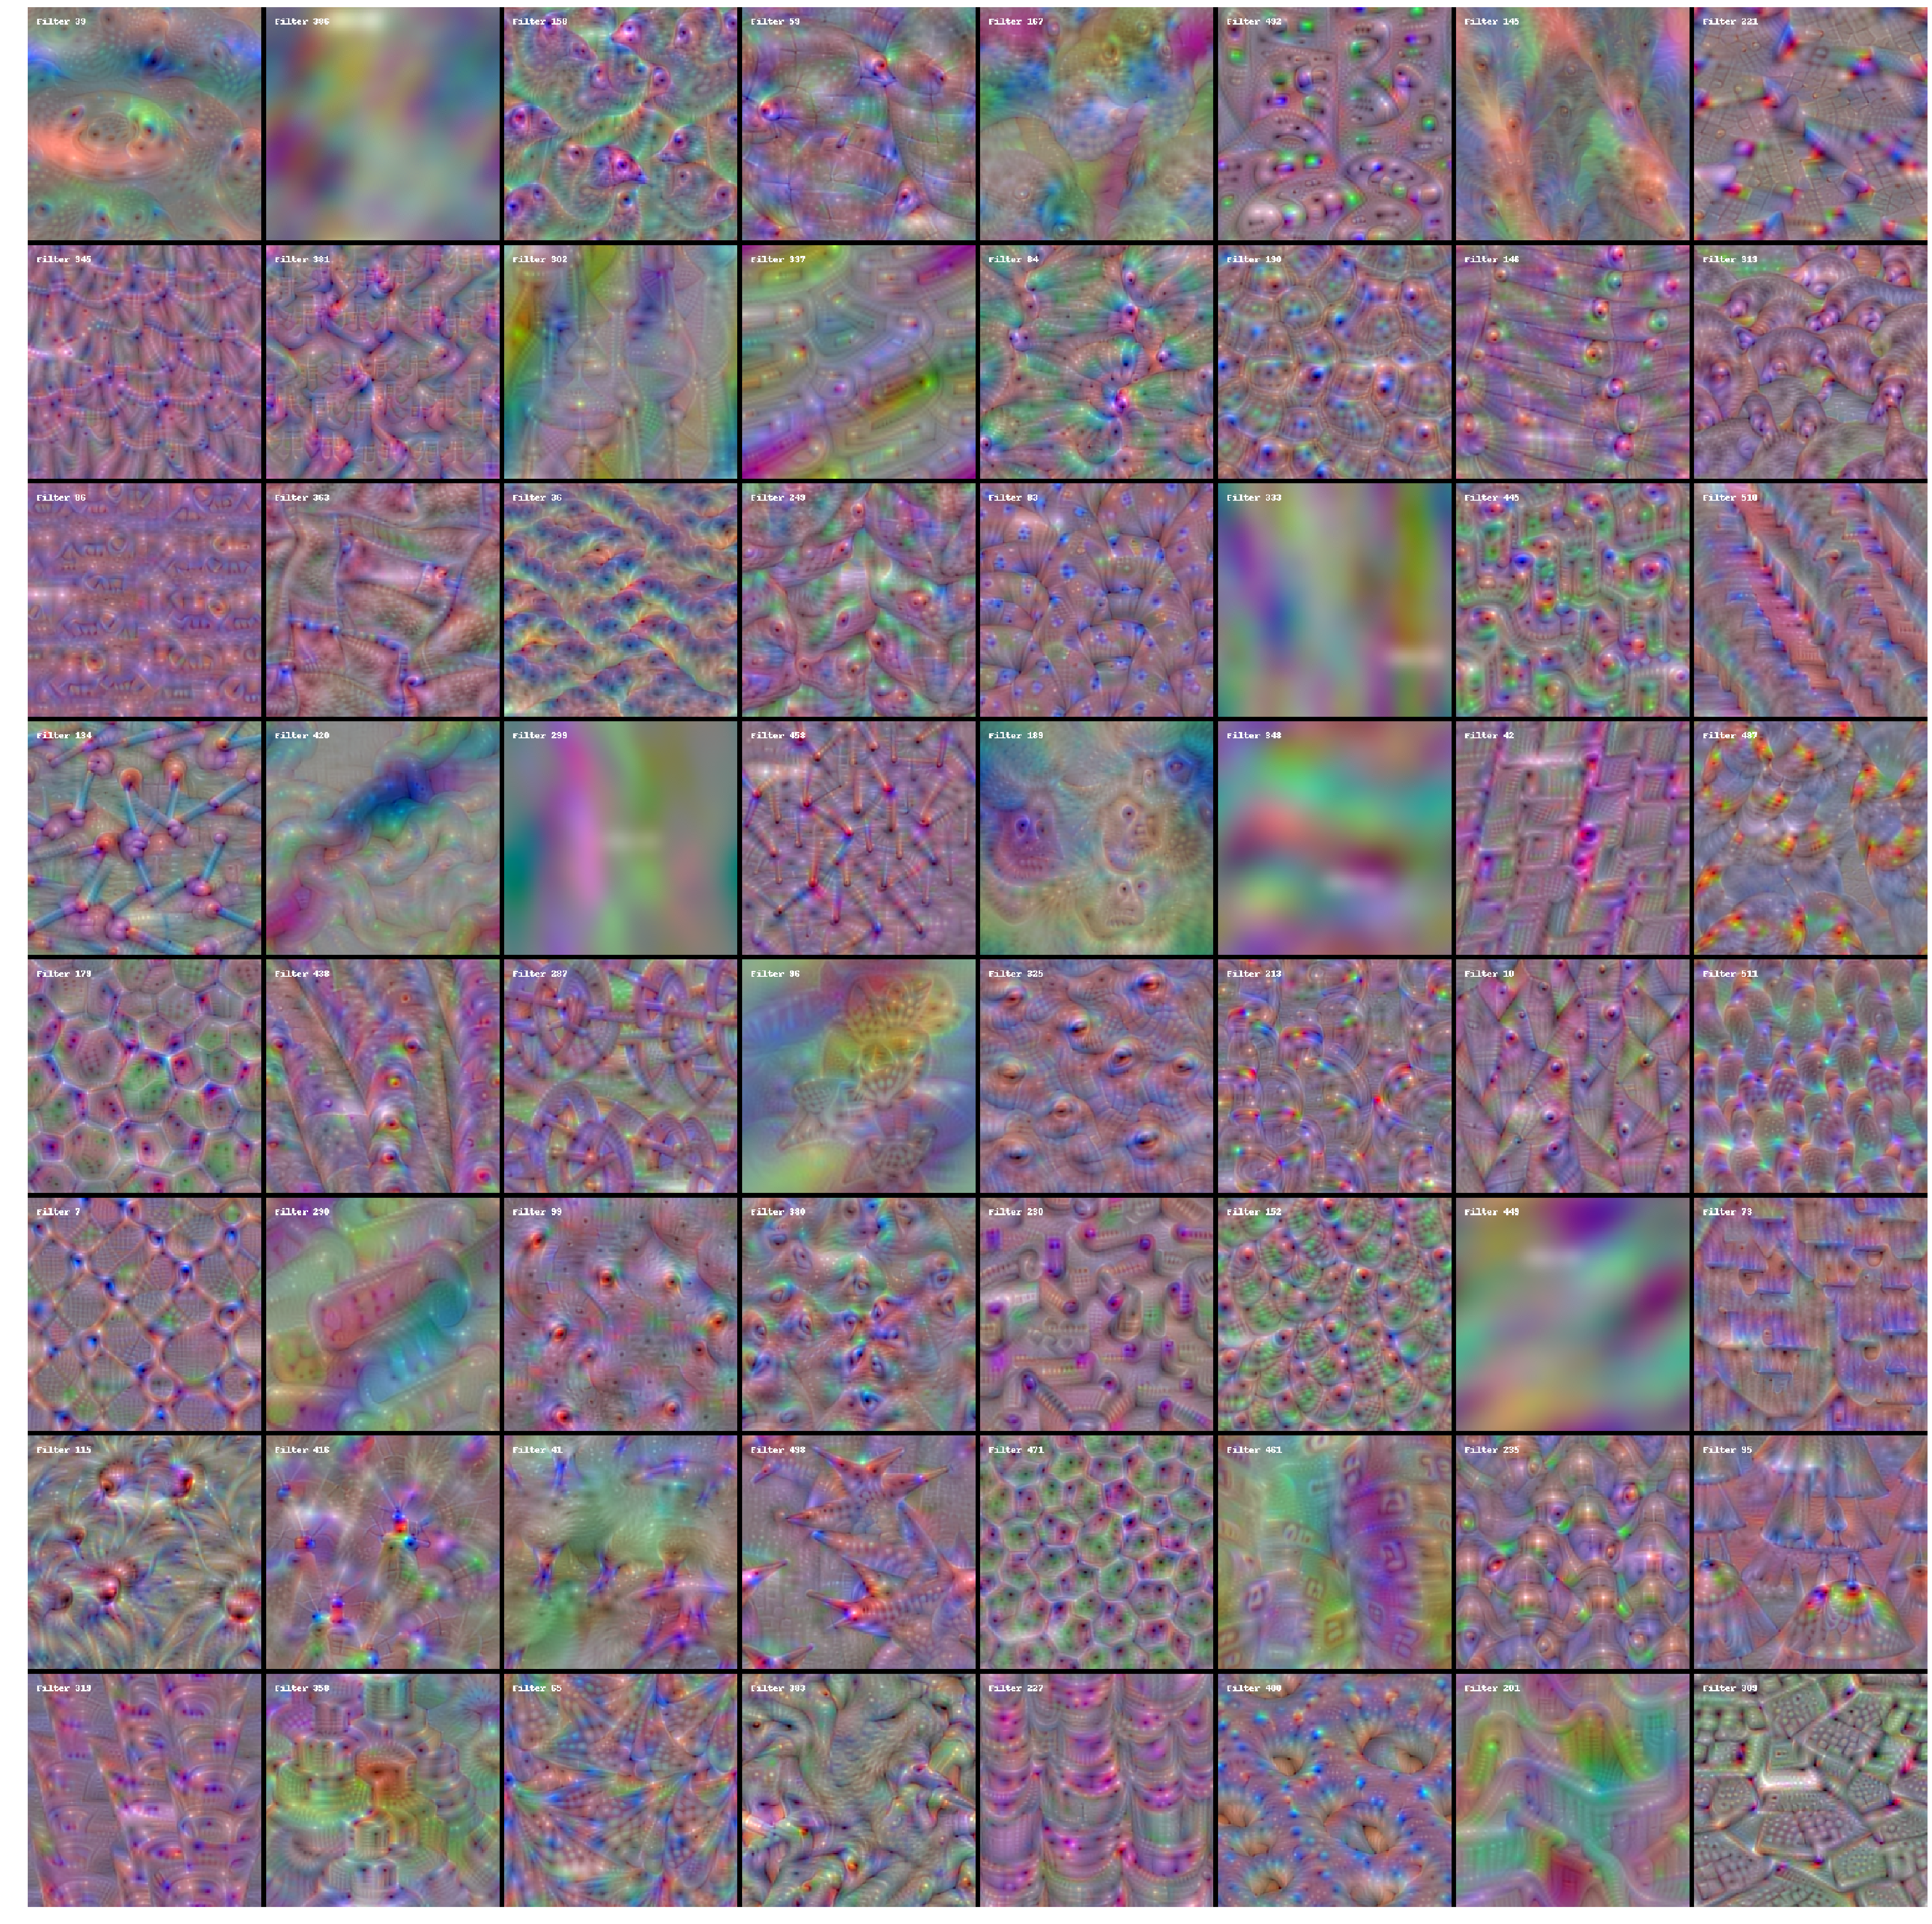
\includegraphics[height=0.95\textheight]{filtros-block5_conv4}
    %     \end{figure}
    %     \pnote{Patrones sumamente complehjos como texturas o regiones}
    % \end{frame}

    \begin{frame}{Comprobación de supuestos}{Mapas de prominencia}
    \begin{columns}
    \column{.38\textwidth}
        \includegraphics[width=\columnwidth,height=0.95\columnwidth]{muestras_saliency.pdf}

        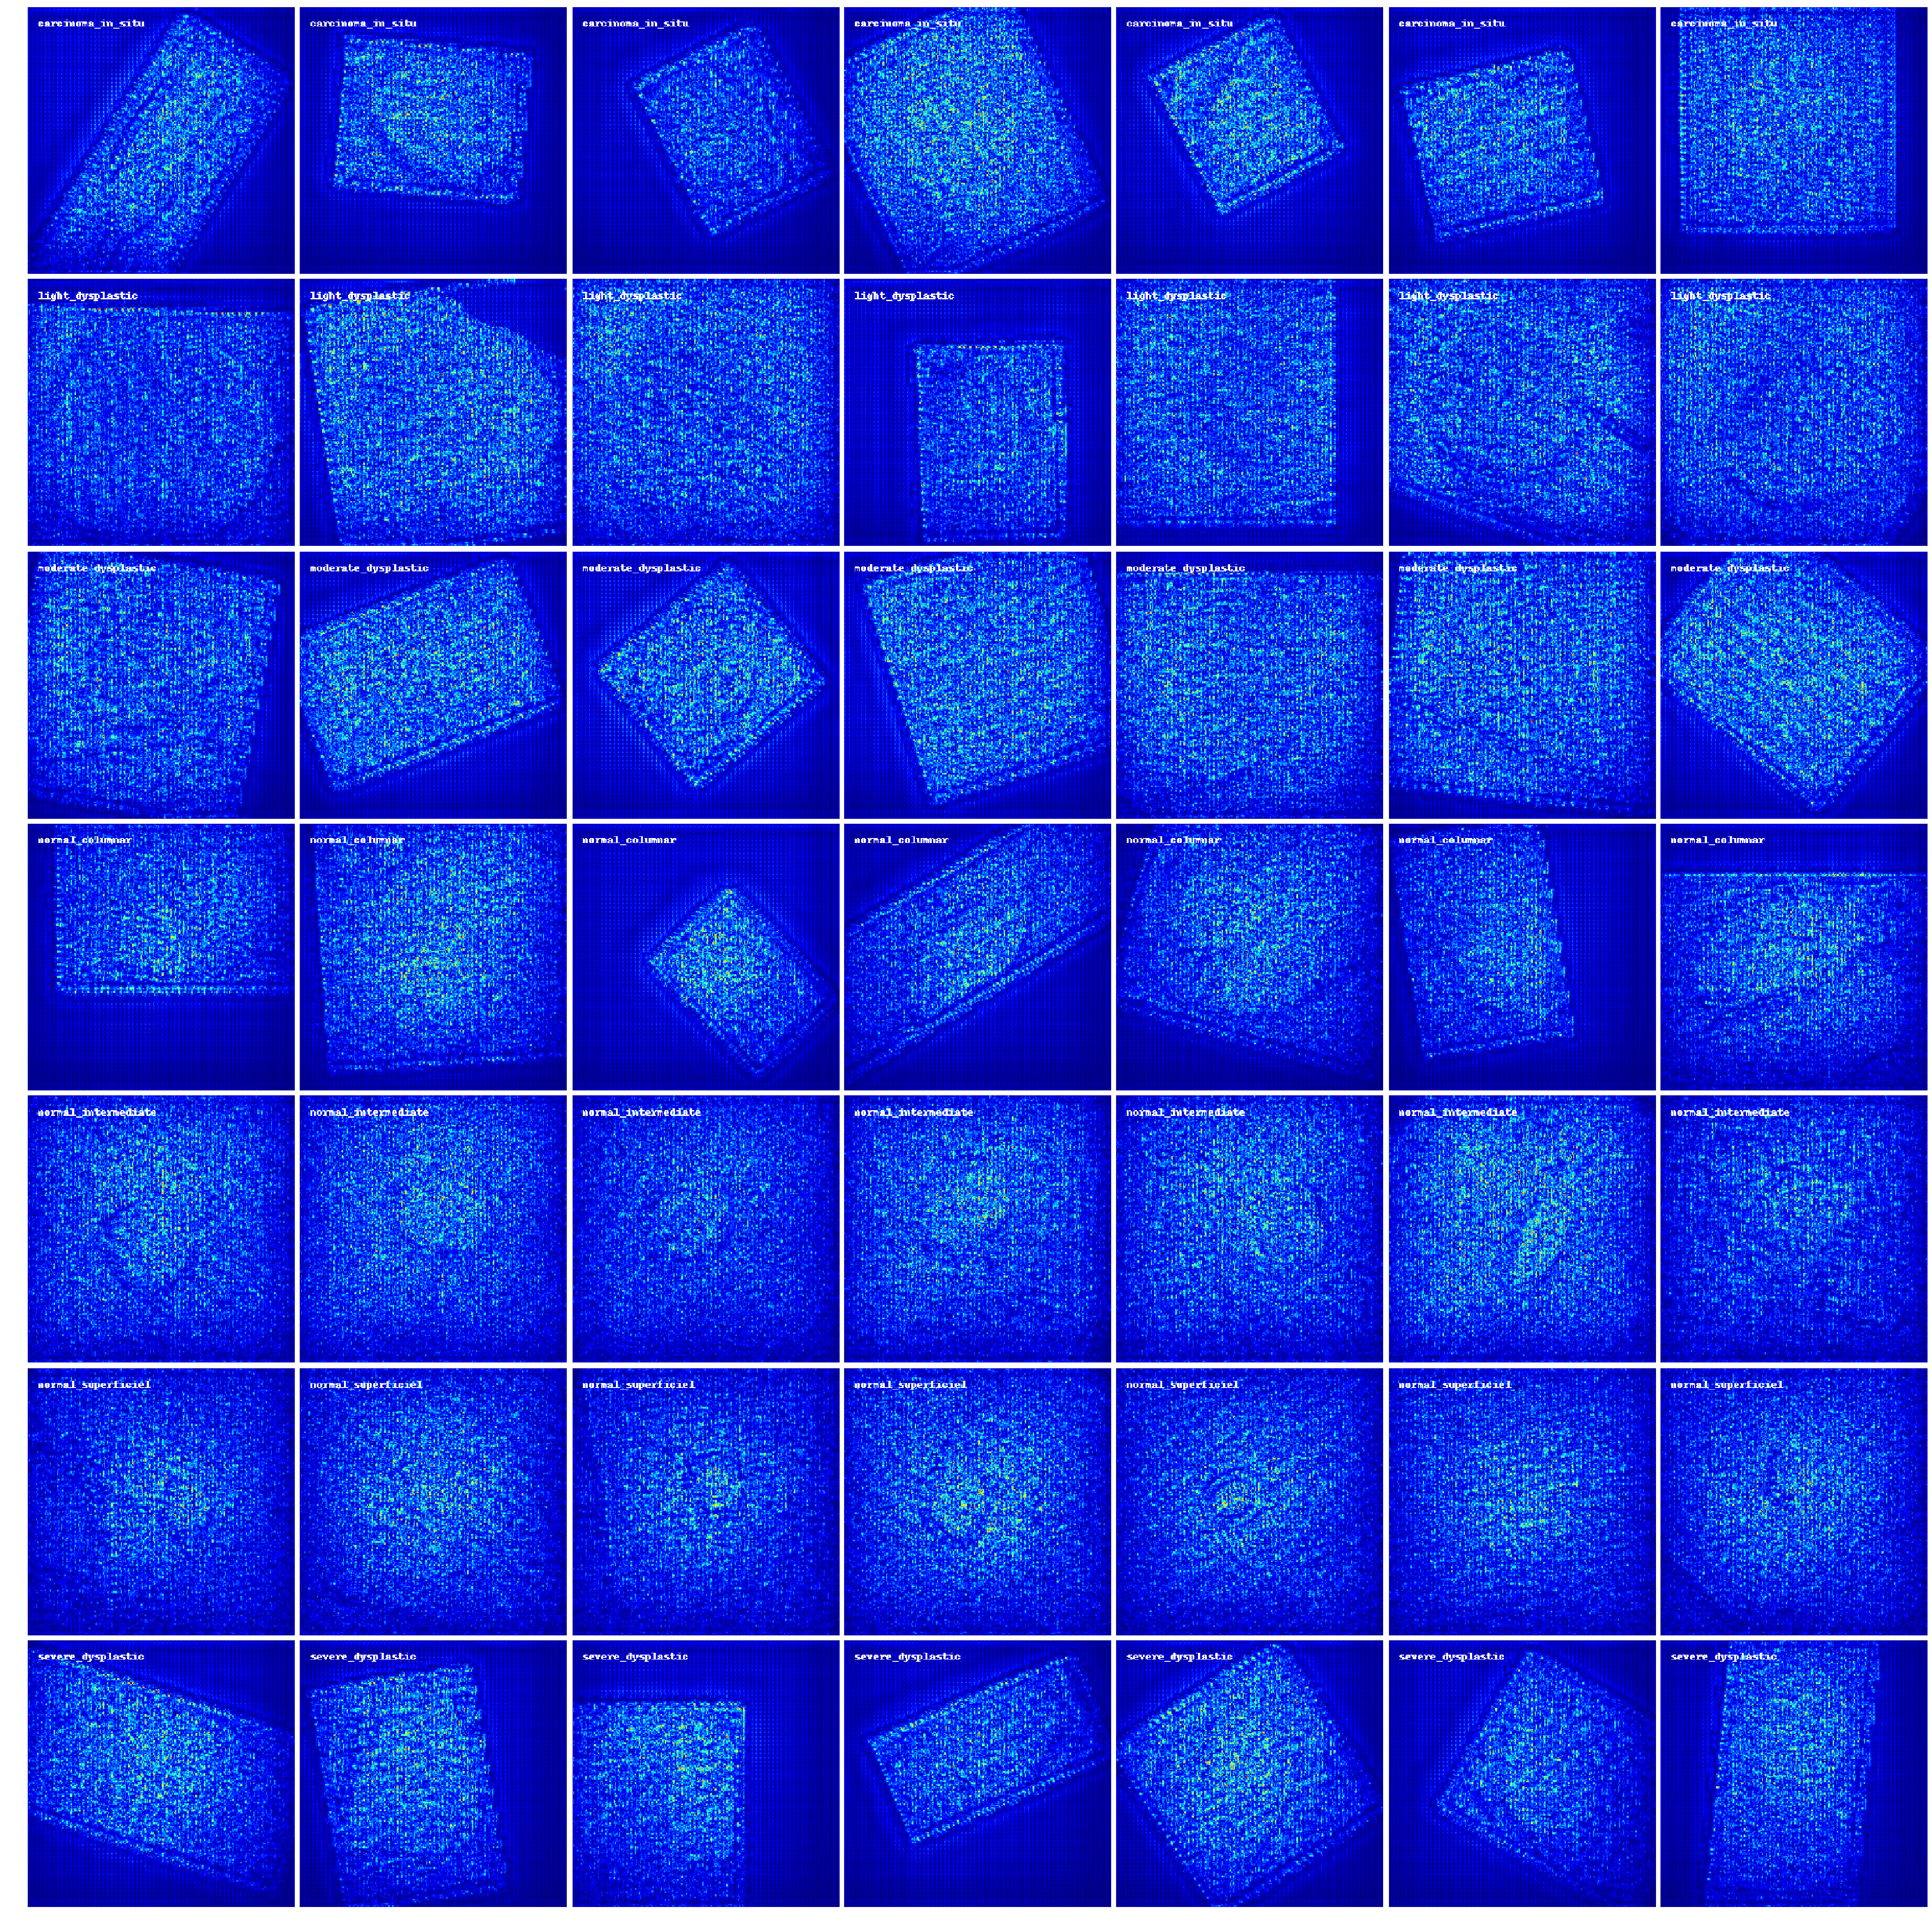
\includegraphics[width=\columnwidth,height=0.95\columnwidth]{saliency_relu.pdf}

        \column{.38\textwidth}
        \includegraphics[width=\columnwidth,height=0.95\columnwidth]{saliency_guided.pdf}

        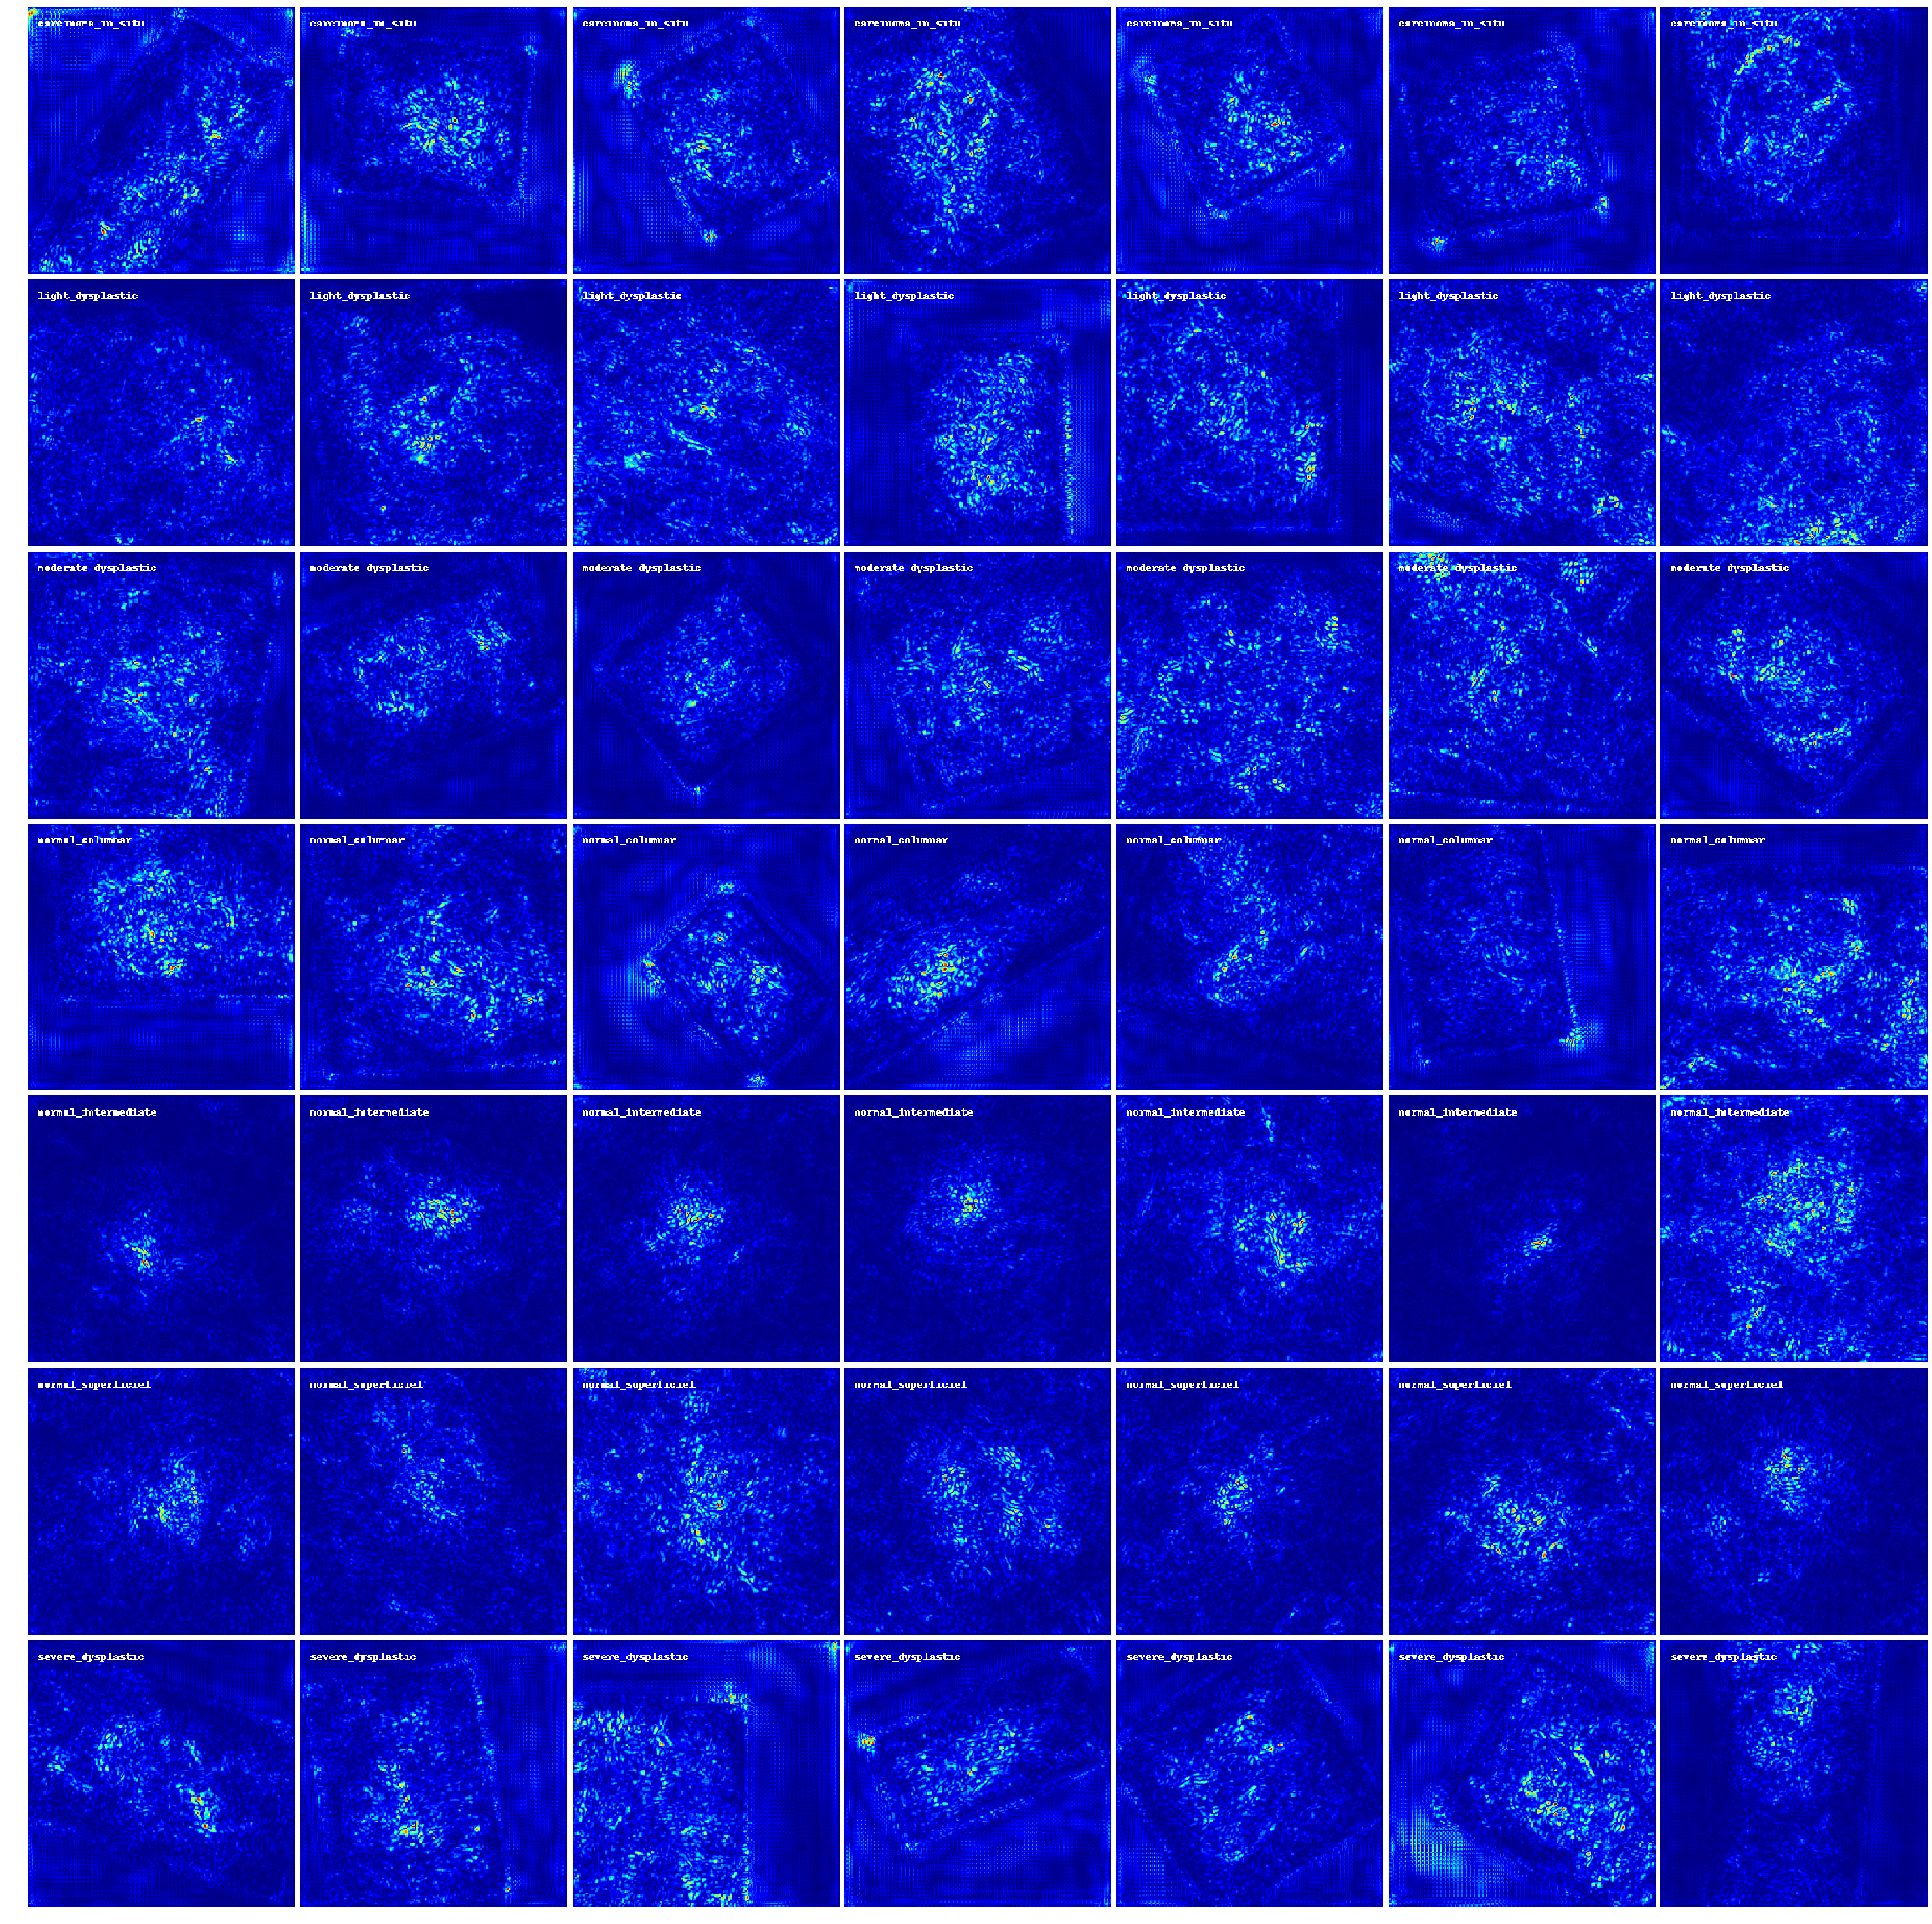
\includegraphics[width=\columnwidth,height=0.95\columnwidth]{saliency_normal.pdf}

    \end{columns}
    \pnote{Es una gráfica de los pixeles que activaron la decisión}
    \pnote{Podemos ver que es la imagen completa y no lo aumentado}
    \pnote{Se centra en el núcleo}
    \end{frame}

    \begin{frame}{Comprobación de supuestos}{Pruebas de oclusión}
        \begin{figure}
            \begin{subfigure}{0.48\textwidth}
            \includegraphics[width=\textwidth]{occlusion-carcinoma_in_situ0.pdf}
            \end{subfigure}\hspace*{\fill}
            \begin{subfigure}{0.48\textwidth}
            \includegraphics[width=\textwidth]{occlusion-light_dysplastic13.pdf}
            \end{subfigure}
    
    
            \begin{subfigure}{0.48\textwidth}
            \includegraphics[width=\textwidth]{occlusion-moderate_dysplastic25.pdf}
            \end{subfigure}\hspace*{\fill}
            \begin{subfigure}{0.48\textwidth}
            \includegraphics[width=\textwidth]{occlusion-normal_columnar34.pdf}
            \end{subfigure}
    
    
            \begin{subfigure}{0.48\textwidth}
            \includegraphics[width=\textwidth]{occlusion-severe_dysplastic64.pdf}
            \end{subfigure}\hspace*{\fill}
            \begin{subfigure}{0.48\textwidth}
            \includegraphics[width=\textwidth]{occlusion-normal_superficiel59.pdf}
            \end{subfigure}
    
            \end{figure}
            \pnote{Se tapan regiones de la imagen para determinar la robustés del modelo}
            \pnote{Se centra en el núcleo}
    \end{frame}

    % \begin{frame}{Comprobación de supuestos}{Reducción de dimensionalidad con \emph{t-sne}}
    %     \begin{figure}[]
    %         \centering
    %         \includegraphics[height=0.95\textheight]{tsne-7clases3-84954-2000.pdf}
    %     \end{figure}
    % \end{frame}

    \begin{frame}{Comparativa de resultados}{Con otros algoritmos aplicados al mismo dataset}
        \begin{table}[]
            \centering
            \resizebox{\textwidth}{!}{%
            \begin{tabular}{@{}lllllll@{}}
            \toprule
            Métodos & k-fold CV & TPR/Sens & TNR/Spec & ACC & F1 & AUC \\ \midrule
            Benchmark & $10$ & \(98.8 \pm 1.3\) & \(79.3 \pm 6.3\) & \(93.6 \pm 1.9\) & $88.0$ & -- \\
            PSO-lnn & $5$ & $98.4$ & $92.2$ & $96.7$ & $95.2$ & -- \\
            GEN-lnn & $5$ & $98.5$ & $92.1$ & $96.8$ & $95.2$ & -- \\
            ANN & -- & $99.9$ & $96.5$ & $99.3$ & $98.2$ & -- \\
            K-PCA + SVM & $5$ & -- & -- & -- & $96.9$ & -- \\
            Ensemble & $5$ & $99$ & $89.7$ & $96.5$ & -- & -- \\
            Ens & $5$ & -- & -- & -- & -- & $0.884$ \\
            dis(S+M) & $5$ & -- & -- & -- & -- & $0.964$ \\
            \rowcolor{azul}
            DeepPap & 5 & \(98.2 \pm 1.2\) & \(98.3 \pm 0.9\) & \(98.3 \pm 0.7\) & \(98.3 \pm 0.3\) & $0.998$ \\
            \rowcolor{verde}
            Tesis binario & 10 & \(0.99857\) & \(0.99979\) & \(99.86\) & \(0.99918\) & $0.99918$ \\ \bottomrule
            \end{tabular}%
            }
            \end{table}

        \begin{block}{Resultados multi-clase}{
            \begin{itemize}
                \item Exactitud DeepPap: $98.5\%$ | Exatitud tesis: $99.58\%$
                \item Error total DeepPap: $1.6\%$ | Error total tesis: $0.42\%$
            \end{itemize}
        }
        \end{block}
    \end{frame}

    \subsection{Implementación}
    \begin{frame}{Plataforma final}{Sistemas embebidos}
        \begin{block}{Características importantes}{
            \begin{itemize}
                \item Bajo costo.
                \item Sin licencias.
                \item Múltiples puertos.
                \item Bajo poder.
                \item Popularidad.
            \end{itemize}
        }
        \end{block}
        \pnote{Instalar el modelo dentro de un sistema de cómputo}
        \pnote{Pequeños dispositivos similares a las computadoras}
    \end{frame}

    % \begin{frame}{Plataforma final}{Nvidia Jetson Nano}
    %     \begin{figure}[]
    %         \centering
    %         \includegraphics[width=1\textwidth]{jetson}
    %     \end{figure}
    %     \pnote{Gran capacidad de procesamiento}
    %     \pnote{Arquitectura pensada para DL y VC}
    % \end{frame}

    % \begin{frame}{Plataforma final}{Rendimiento}
    %     \begin{figure}[]
    %         \centering
    %         \includegraphics[width=1\textwidth]{jetson_comparison}
    %     \end{figure}
    % \end{frame}

    \begin{frame}{Plataforma final}{Componentes del sistema}
        \begin{figure}[]
            \centering
            \includegraphics[height=0.95\textheight]{componentes}
        \end{figure}
        \pnote{Se utiliza una cámara de alta definición}
        \pnote{Una pantalla táctil}
    \end{frame}

    \begin{frame}{Plataforma final}{Adaptador cámara-microscópio impreso en 3D}
        \begin{figure}[]
            \centering
            \includegraphics[height=0.95\textheight]{adaptador_final}
        \end{figure}
        \pnote{Para conectar la cámara al microscopio}
    \end{frame}

    \begin{frame}{Plataforma final}{Carcasa del dispositivo impresa en 3D}
        \begin{columns}
            \column{.5\textwidth}
            \includegraphics[width=\columnwidth,height=\columnwidth]{large_preview_front}
    
            \column{.5\textwidth}
            \includegraphics[width=\columnwidth,height=\columnwidth]{large_preview_back}
        \end{columns}
        \pnote{De bajo costo y para ser usada dentro del laboratorio}
    \end{frame}

    \begin{frame}{Plataforma final}{Muestra del prototipo}
        \begin{figure}[]
            \centering
            \includegraphics[height=0.95\textheight]{prototipo_final}
        \end{figure}
        \pnote{Se puede ver una prueba del sistema ya instalado}
    \end{frame}

    \begin{frame}{Plataforma final}{Pantalla de inicio del software}
        \begin{figure}[]
            \centering
            \includegraphics[height=0.95\textheight]{gui}
        \end{figure}
    \end{frame}

    \begin{frame}{Plataforma final}{Ejemplo de uso del software}
        \begin{figure}[]
            \centering
            \includegraphics[height=0.95\textheight]{gui2}
        \end{figure}
        \pnote{Podemos ver que da una pribabilidad de pertenencia a cierta clase}
    \end{frame}

    \section{Resultados}
    \begin{frame}{Resultados}{Tabla de resultados de los experimentos}
        \begin{table}[]
            \centering
            \resizebox{1\textwidth}{!}{%
            \begin{tabular}{@{}lll@{}}
            \toprule
            \textbf{Experimento} & \textbf{Exactitud} & \textbf{Pérdida} \\ \midrule
            \rowcolor{azul}
            Binario & 99.86\% & 0.0038 \\
            \rowcolor{verde}
            Multi-clase & 99.58\% & 0.013 \\
            \rowcolor{media}
            Segmentación & 90.20\% & -0.9 \\ \bottomrule
            \end{tabular}%
            }
        \end{table}
    \end{frame}


    \subsection{Replicabilidad del experimento}
    \begin{frame}{Diseño experimental}{Disposiciones para repetir, reproducir y replicar el experimento}
        \begin{block}{Características}{
            \begin{enumerate}
                \item{\textbf{Repetible:}} Es la capacidad de volver a hacer el experimento
                en otro entorno ajeno al del investigador original y con un código
                independiente al entorno inicial de investigación.
                \item{\textbf{Reproducible:}} Un estudio es reproducible si se pueden tomar
                los datos originales y el código computacional usado para analizarlos y
                reproducir todos los hallazgos numéricos del estudio.
                \item{\textbf{Replicable:}} Es el acto de repetir un estudio completo,
                independientemente del investigador original sin el uso de datos originales
                y utilizando los mismos métodos.
            \end{enumerate}
        }
        \end{block}
        \pnote{Es por ello que se trabajó arduamente para generar las disposiciones y documentación para cumplir}
    \end{frame}

    \begin{frame}{Repositorios de código}{Ingeniería de Software como metodología de experimentación}
        \begin{figure}[]
            \centering
            \includegraphics[height=0.95\textheight]{git}
        \end{figure}
    \end{frame}

    \begin{frame}{\emph{Jupyter Notebooks}}{Un nuevo modo de hacer análisis de datos}
        \begin{figure}[]
            \centering
            \includegraphics[width=\textwidth, height=0.95\textheight]{note}
        \end{figure}
    \end{frame}

    \subsection{Trabajo a futuro}

    \begin{frame}{Trabajo a futuro}{Detección}
        \begin{figure}[]
            \centering
            \includegraphics[height=0.95\textheight]{object}
        \end{figure}
    \end{frame}

    \begin{frame}{Trabajo a futuro}{Instanciación}
        \begin{figure}[]
            \centering
            \includegraphics[width=1\textwidth]{ejemplo}
        \end{figure}
    \end{frame}
    \begin{frame}{Trabajo a futuro}{Despliegue: Convertir un sistema en una solución}
        \begin{figure}[]
            \centering
            \includegraphics[height=0.95\textheight]{despliegue}
        \end{figure}
        \pnote{Un sistema no es una solución}
        \pnote{S erequiere preparar para su uso en producción}
    \end{frame}

    \begin{frame}{Trabajo a futuro}{Sistema ciber-físico}
        \begin{figure}[]
            \centering
            \includegraphics[height=0.95\textheight]{cloud}
        \end{figure}
        \pnote{El experto puede interactuar con el sistema}
        \pnote{Avisar de errores de clasificación}
        \pnote{Capturar imágenes para reentrenar el sistrema}
    \end{frame}


    \subsection{Conclusiones}
    \begin{frame}{Conclusiones}{}
        \begin{exampleblock}{Comentarios finales}{
            \begin{itemize}
                \item Detectar a tiempo el cáncer es crucial.
                \item La clasificación multi-clase ofrece más información al experto.
                \item Es importante evaluar correctamente el modelo.
                \item Se necesita saber como el algoritmo toma las decisiones.
                \item Conjugar la experiencia del experto con el algoritmo es la clave.
                \item Usar Deep Learning simplifica mucho el trabajo.
                \item Auxiliarse de técnicas de \emph{Industria 4.0} acelera el prototipado.
            \end{itemize}
        }
            
        \end{exampleblock}
    \end{frame}

    \section{Productividad}
    \begin{frame}{Sistema de información geográfica}{Reducción de riesgo obstétrico por dengue}
        \begin{figure}[]
            \centering
            \includegraphics[width=\textwidth]{gis}
        \end{figure}
    \end{frame}
    \subsection{Sistema de información geográfica}
    \begin{frame}{Sistema de información geográfica}{Ponencia en congreso}
        \begin{block}{Descripción}{
            \begin{itemize}
                \item Congreso Internacional de Logística y Cadena de Suministro
                \item 10 a 12 de Octubre, Palacio de Minería, Ciudad de México.
                \item Marco J. Del Moral-Argumedo, Alberto A. Aguilar-Lasserre,
                Carlos F. Vázquez-Rodríguez.
            \end{itemize}
        }
        \end{block}
        \begin{figure}[]
            \centering
            \includegraphics[width=\textwidth]{cilog}
        \end{figure}
    \end{frame}

    \begin{frame}{Sistema de información geográfica}{Capítulo en libro}
        \begin{figure}[]
            \centering
            \includegraphics[height=0.95\textheight]{libro}
        \end{figure}
    \end{frame}

    \subsection{Estancias}
    \begin{frame}{Estancia internacional de investigación}{Metaheurísticas para optimización de algoritmos de Deep Learning}
        \begin{columns}
            \column{.5\textwidth}
            \includegraphics[width=\columnwidth,height=\columnwidth]{lgc}
    
            \column{.5\textwidth}
            \includegraphics[width=\columnwidth,height=\columnwidth]{inp}
        \end{columns}
    \end{frame}

    \subsection{Registros y patentes}
    \begin{frame}{Registros y patentes}{Asegurando la propiedad intelectual}
        \begin{columns}
            \column{.5\textwidth}
            \includegraphics[width=\columnwidth,height=\columnwidth]{impi}
    
            \column{.5\textwidth}
            \includegraphics[width=\columnwidth,height=\columnwidth]{indautor}
        \end{columns}
    \end{frame}

    \subsection{Premios}

    \begin{frame}{Olimpiadas de la Innovación}{Instituto Mexicano del Seguro Social}
        \begin{figure}[]
            \centering
            \includegraphics[width=\textwidth, height=0.95\textheight, keepaspectratio]{olimpiadas}
        \end{figure}
    \end{frame}


    \begin{frame}{Premio a la Innovación Tecnológica}{Sistema de Transporte Colectivo Metro}
        \begin{figure}[]
            \centering
            \includegraphics[width=\textwidth]{medalla}
        \end{figure}
    \end{frame}

    \subsection{Artículos}
    \begin{frame}{Artículo JCR (2.217)}{Multi-agent systems}
        \begin{columns}
            \column{.5\textwidth}
            \includegraphics[width=\columnwidth]{mdpi}
    
            \column{.5\textwidth}
            \begin{block}{Autores}{
                \begin{itemize}
                    \item María del Rosario Pérez-Salazar.
                    \item Alberto Alfonso Aguilar-Lasserre.
                    \item Rubén Posada-Gómez.
                    \item Marco J. Del Moral-Argumedo.
                    \item José Carlos Hernández-González.
                    \item Miguel Gastón Cedillo-Campo.
                \end{itemize}
            }
                
            \end{block}
        \end{columns}
    \end{frame}

    \subsection{Donaciones}
    \begin{frame}{Donaciones}{Un sueño hecho realidad}
        \begin{figure}[]
            \centering
            \includegraphics[width=\textwidth]{titan}
        \end{figure}
    \end{frame}

    \subsection{Otros}
    \begin{frame}{Otros proyectos y participaciones}{Programador bajo demanda}
        \begin{exampleblock}{Participaciones}{
            \begin{itemize}
                \item Desarrollo de Sistema Experto para catación de café.
                \item Desarrollo de Sistema Experto para generación de biogas.
                \item Desarrollo de Sistema de Información Geográfica para logística humanitaria.
                \item Desarrollo de Sistema Experto para análisis de riesgo diabético.
                \item Desarrollo de Sistema de Información Geográfica para
                consultoría en análisis de mantos acuíferos.
                \item Desarrollo de Sistema Experto para predecir el comportamiento del cliente.
            \end{itemize}
        }
        \end{exampleblock}
    \end{frame}

    % \section{Agradecimientos}
    \begin{frame}
        \frametitle{¡Muchas gracias!}
        \begin{figure}[]
            \centering
            \includegraphics[height=0.95\textheight]{thanks}
        \end{figure}
    \end{frame}

\end{document}